\documentclass{beamer}
\usepackage{../common_slides}
\usepackage{tikz}
\usepackage{tikz-qtree}
\usepackage{pdfpages}


\usetikzlibrary{bayesnet,matrix}
% \usepackage{enumitem}
\tikzstyle{hid}=[draw]
\tikzstyle{obs}=[draw]


\title{Question Answering/Semantic Parsing}
\date{}
\author{CS 287 \\ (Slides from Yoav Artzi)}

\begin{document}
\begin{frame}
  \titlepage
\end{frame}

% \begin{frame}{Review:}
%   \begin{center}
%     \begin{tikzpicture}
%       \matrix (network) [matrix of nodes, ampersand replacement=\&,
%       column sep={1cm},
%       row sep={1cm}] {
%         \& \& \& \node{the}; \& \node{red}; \& \node{dog}; \\
%         \& \& \& \node[obs]{$\hat{\boldy}_1$}; \& \node[obs]{$\hat{\boldy}_2$}; \& \node[obs]{$\hat{\boldy}_3$}; \\
%         \node[hid]{$\bolds^s_1$}; \& \node[hid]{$\bolds^s_2$}; \& \node[hid]{$\bolds^s_3$}; \& \node[hid]{$\bolds^t_1$}; \& \node[hid]{$\bolds^t_2$}; \& \node[hid]{$\bolds^t_3$}; \\
%         \node[obs]{$\boldx_1$}; \& \node[obs]{$\boldx_2$}; \& \node[obs]{$\boldx_3$};  \&   \node[obs]{$\hat{\boldx}_1$}; \& \node[obs]{$\hat{\boldx}_2$}; \& \node[obs]{$\hat{\boldx}_3$}; \\
%           \node[obs]{the}; \& \node[obs]{red}; \& \node[obs]{dog};  \&  \node[obs]{$<$s$>$}; \&  \&  \\
%       }; 


%       \draw[->] (network-5-1) -- (network-4-1); 
%       \draw[->] (network-5-2) -- (network-4-2); 
%       \draw[->] (network-5-3) -- (network-4-3);
%       \draw[->] (network-5-4) -- (network-4-4);


%       \draw[->] (network-4-1) -- (network-3-1); 
%       \draw[->] (network-4-2) -- (network-3-2); 
%       \draw[->] (network-4-3) -- (network-3-3);


%       \draw[->] (network-3-1.east) -- (network-3-2.west); 
%       \draw[->] (network-3-2.east) -- (network-3-3.west); 
%       \draw[->] (network-3-3.east) -- (network-3-4.west); 



      
%       \draw[->] (network-1-4) -- (network-4-5.west); 
%       \draw[->] (network-1-5) -- (network-4-6.west); 

%       \draw[->] (network-3-4.east) -- (network-3-5.west); 
%       \draw[->] (network-3-5.east) -- (network-3-6.west); 

%       \draw[->] (network-2-4) -- (network-1-4); 
%       \draw[->] (network-2-5) -- (network-1-5); 
%       \draw[->] (network-2-6) -- (network-1-6);

%       \draw[->] (network-4-4) -- (network-3-4); 
%       \draw[->] (network-4-5) -- (network-3-5); 
%       \draw[->] (network-4-6) -- (network-3-6);

%       \draw[->] (network-3-4) -- (network-2-4); 
%       \draw[->] (network-3-5) -- (network-2-5); 
%       \draw[->] (network-3-6) -- (network-2-6);

%     \end{tikzpicture}
%   \end{center}

% \end{frame}



\begin{frame}{Question}
  It has become a popular strategy to handle 
  sequential prediction problems using a seq2seq setup
  such as attention-based translation. How might you 
  handle the following problems: 

  \begin{enumerate}
  \item Segmentation (HW4)
  \item Rare Word Replacement (HW3)
  \item Part-of-Speech Tagging (HW2-HW5)
  \end{enumerate}
\end{frame}

\begin{frame}{Today's Lecture}
  Question Answering 
  \begin{itemize}
  \item Semantic Parsing: linguistic-model of questions and answers
    \air
  \item Knowledge Base and Dataset
    \air 
    
  \item Watson and Jeopardy!
  \end{itemize}
  
\end{frame}

{
\setbeamercolor{background canvas}{bg=}
\includepdf[pages=4]{jobslides.pdf}
}

{
\setbeamercolor{background canvas}{bg=}
\includepdf[pages=93]{artzitut.pdf}
}


\section{Freebase/Wikidata}

\begin{frame}
  \begin{center}
    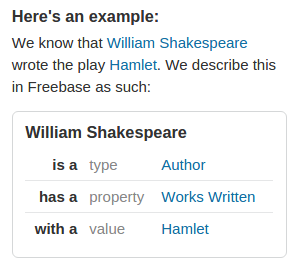
\includegraphics[width=5cm]{freebase}
  \end{center}
\end{frame}

\begin{frame}
  \begin{center}
    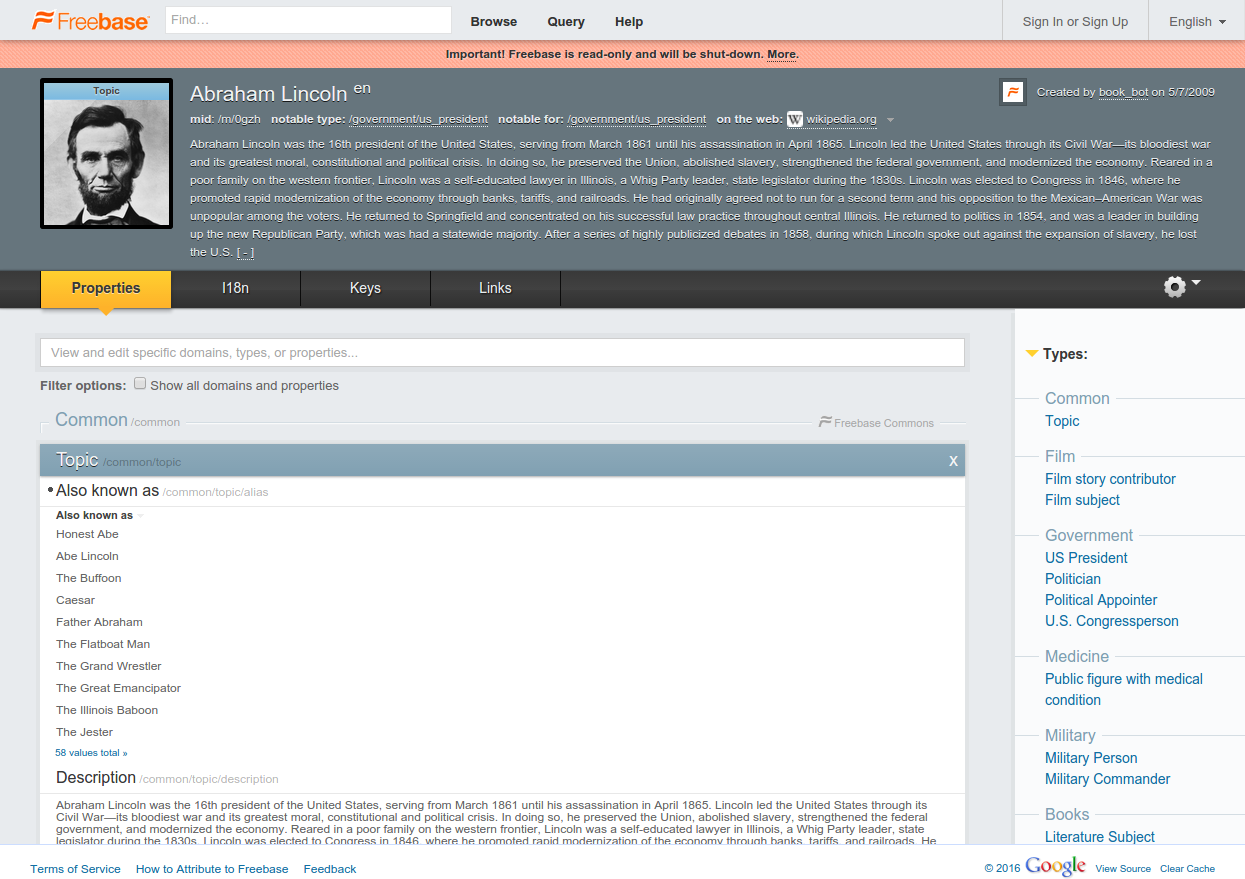
\includegraphics[width=\textwidth]{freebaseabe}
  \end{center}
\end{frame}

\begin{frame}
  \begin{center}
    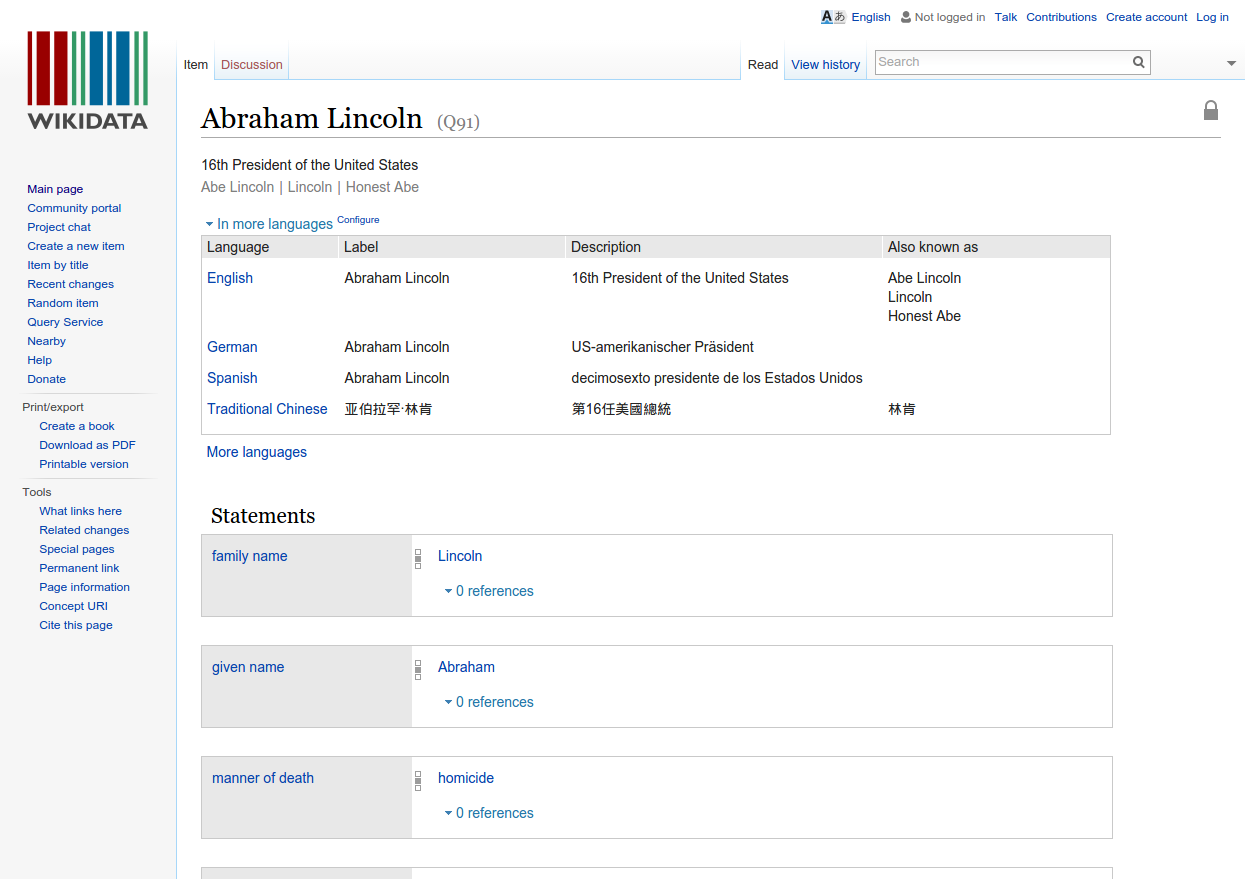
\includegraphics[width=\textwidth]{wikiabe}
  \end{center}
\end{frame}


\section{Semantic Parsing}

\begin{frame}
  
\end{frame}

{
\setbeamercolor{background canvas}{bg=}
\includepdf[pages=5-6]{artzitut.pdf}
}


{
\setbeamercolor{background canvas}{bg=}
\includepdf[pages=8-11]{artzitut.pdf}
}


{
\setbeamercolor{background canvas}{bg=}
\includepdf[pages=23-41]{artzitut.pdf}
}

{
\setbeamercolor{background canvas}{bg=}
\includepdf[pages=97-99]{artzitut.pdf}
}

{
\setbeamercolor{background canvas}{bg=}
\includepdf[pages=100-104]{artzitut.pdf}
}


\section{Data Sets}

\begin{frame}{Geoquery (Zelle and Mooney, 1996)}
  \begin{center}
    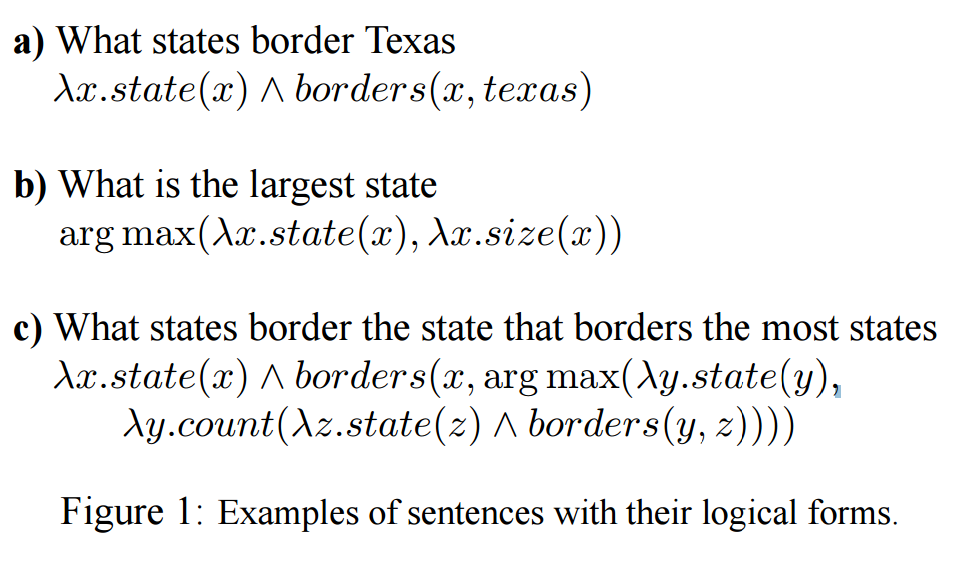
\includegraphics[width=10cm]{geoquery}
  \end{center}
\end{frame}

\begin{frame}[fragile]{WebQuestions (Berant, 2013)} 
\textbf{Questions:}
\begin{itemize}
\item what high school did president bill clinton attend?
\item what form of government does russia have today?
\item what movies does taylor lautner play in?
\end{itemize}
\textbf{Answers:}
\begin{itemize}
\item Hot Springs High School \url{http://www.freebase.com/view/en/bill_clinton}
\item Constitutional republic \url{http://www.freebase.com/view/en/russia}
\item  Eclipse, Valentine's Day, The Twilight Saga: Breaking Dawn -   Part 1, New Moon \url{http://www.freebase.com/view/en/taylor_lautner}
\end{itemize}


\end{frame}

\begin{frame}{WebQuestions}
  \begin{quote}
    To collect this dataset, we used the Google Suggest API to obtain
    questions that begin with a whword and contain exactly one
    entity. We started with the question “Where was Barack Obama
    born?”  and performed a breadth-first search over questions
    (nodes), using the Google Suggest API supplying the edges of the
    graph. Specifically, we queried the question excluding the entity,
    the phrase before the entity, or the phrase after it; each query
    generates 5 candidate questions, which are added to the queue.  We
    iterated until 1M questions were visited; a random 100K were
    submitted to Amazon Mechanical Turk.
  \end{quote}
\end{frame}

\begin{frame}{WebQuestions}
  \begin{quote}
    The AMT task requested that workers answer the question using only
    the Freebase page of the questions’ entity, or otherwise mark it
    as unanswerable by Freebase. The answer was restricted to be one
    of the possible entities, values, or list of entities on the
    page. As this list was long, we allowed the user to filter the
    list by typing. We paid the workers \$0.03 per question. Out of
    100K questions, 6,642 were annotated identically by at least two
    AMT workers.
  \end{quote}
\end{frame}

\begin{frame}
  \begin{center}
    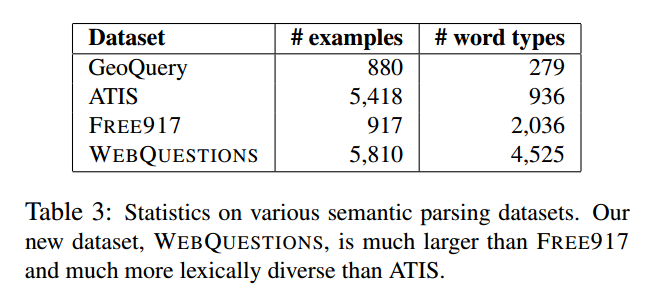
\includegraphics[width=10cm]{webquestions}
  \end{center}
\end{frame}

\section{Jeopardy!}

\begin{frame}
  \begin{center}
    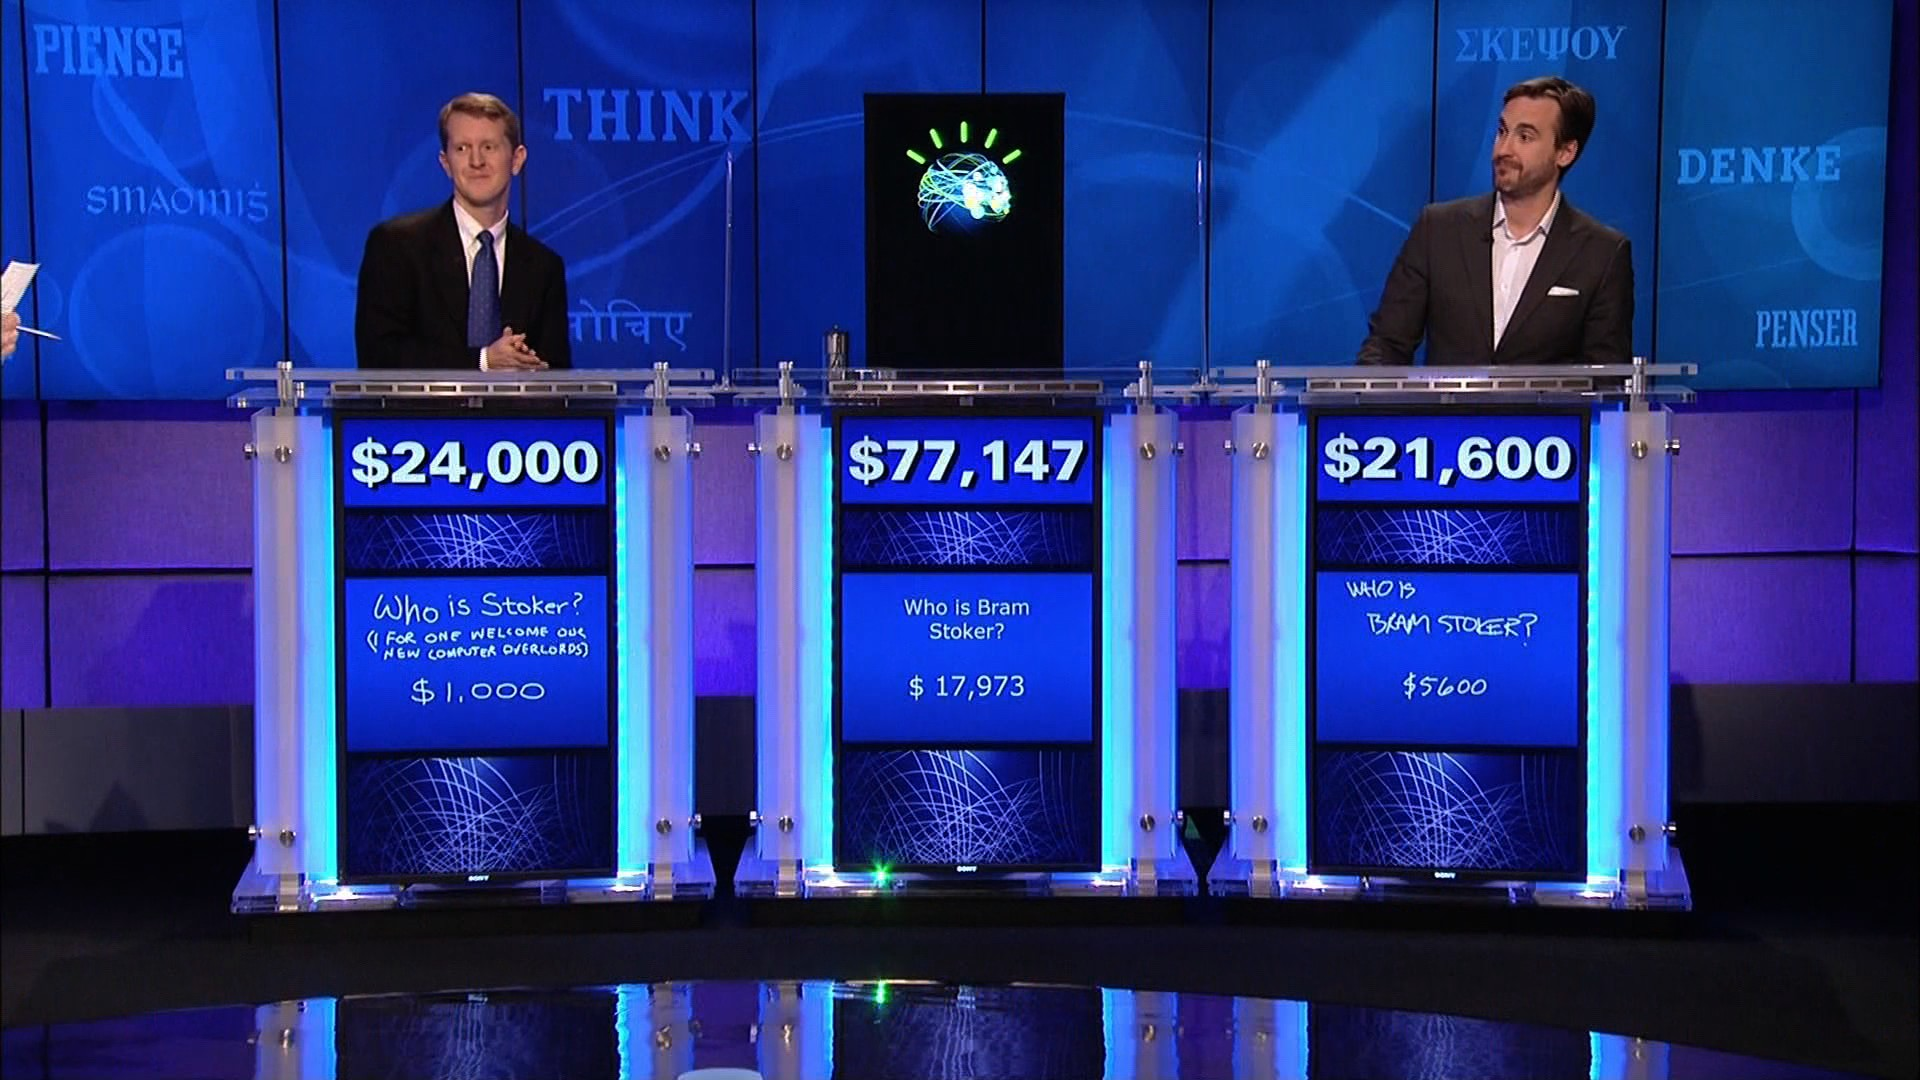
\includegraphics[width=10cm]{IBMwatson}
  \end{center}
\end{frame}

\begin{frame}{DeepQA}
  \begin{itemize}
  \item (not actually deep learning)
  \end{itemize}
\end{frame}

\begin{frame}
  \begin{center}
    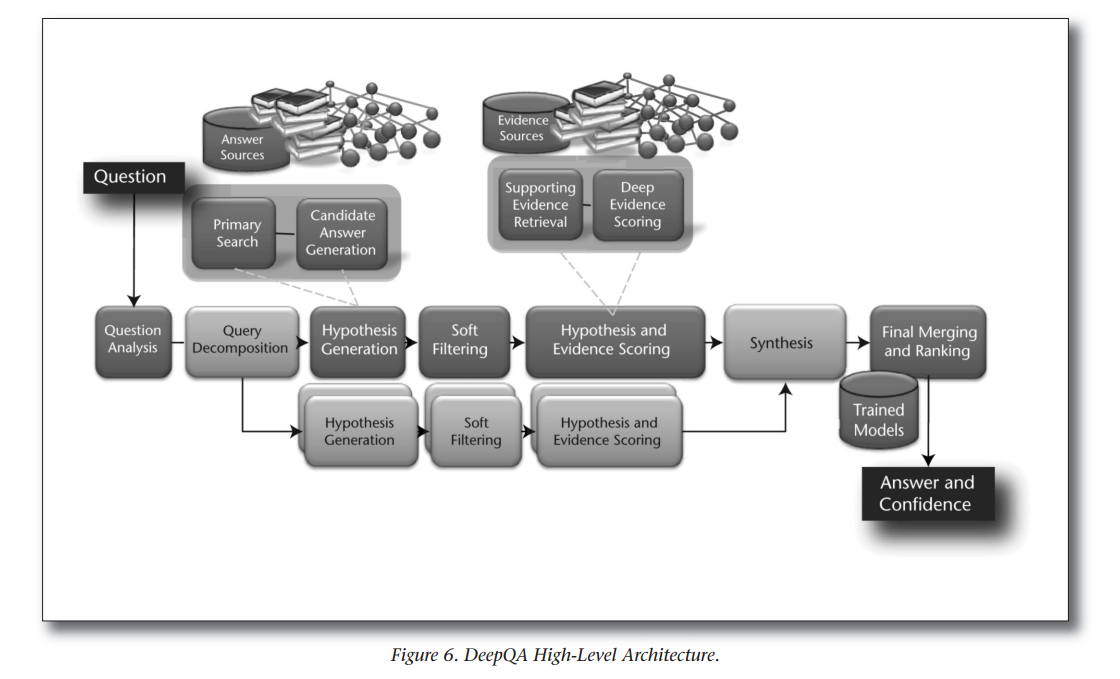
\includegraphics[width=10cm]{deepqa}
  \end{center}
\end{frame}

\begin{frame}{Candidate Generation}
  
\end{frame}

\begin{frame}
  \begin{quote}
    This motivates an approach that merges answer scores before
    ranking and confidence estimation.  Using an ensemble of matching,
    normalization, and coreference resolution algorithms, Watson
    identifies equivalent and related hypotheses (for example, Abraham
    Lincoln and Honest Abe) and then enables custom merging per
    feature to combine scores.
  \end{quote}
\end{frame}

\begin{frame}
  \begin{quote}
    Given the kinds of questions and broad domain of the Jeopardy
    Challenge, the sources for Watson include a wide range of
    encyclopedias, dictionaries, thesauri, newswire articles, literary
    works, and so on.
  \end{quote}
\end{frame}

\begin{frame}
  \begin{quote}
    A variety of search techniques are used, including the use of
    multiple text search engines with different underlying approaches
    (for example, Indri and Lucene), document search as well as
    passage search, knowledge base search using SPARQL on triple
    stores, the generation of multiple search queries for a single
    question, and backfilling hit lists to satisfy key constraints
    identified in the question.
  \end{quote}
\end{frame}

\begin{frame}{Hypothesis Ranking}
  \begin{center}
    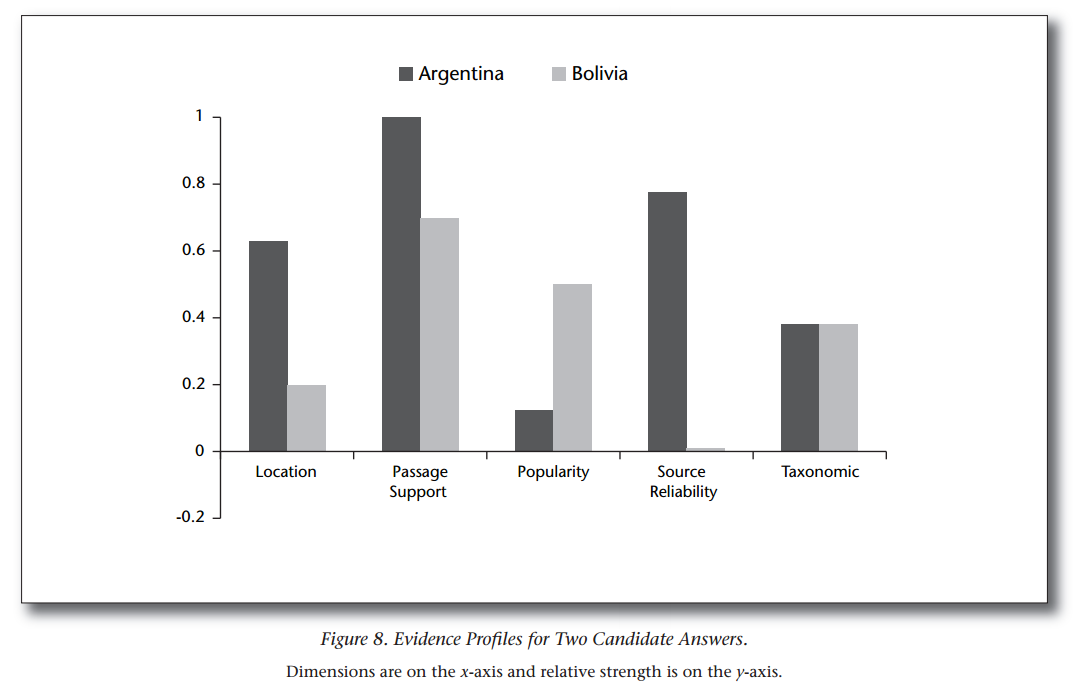
\includegraphics[width=10cm]{deepqaanalysis}
  \end{center}
\end{frame}

\begin{frame}{Other Aspects}
  \begin{itemize}
  \item Parsing algorithm
    \air 
  \item Inducing rules and parameters
    \air 
  \item Relationship between syntax and semantics
  \end{itemize}
\end{frame}

{
\setbeamercolor{background canvas}{bg=}
\includepdf[pages=48-53]{artzitut.pdf}
}

\end{document}